\subsection{Exploratory Search}
The search for information and extending one's knowledge is a built-in behaviour in humans.
Last few decades have transformed search and made it an everyday function.
It wasn't until the late 1990's until web search services began offering quick access to information and changed the ways of information seeking.
Before the Web, information search services were used mainly by academics and information professionals.
With a small amount of users, the search system manufacturers didn't need to focus on the user experience and motivation to improve the user interface was .
Traditional search systems were lookup-based and as such, the query formulation was an essential stage of the search task.
Some studies mention systems, where the query results took days to return . In such cases, the (user learns the system very slowly), since becoming a better user of such a system requires interaction with system and slow (query return) means slow learning.

Search system must be quick for other reasons too. Cognitive abilities restrict the searcher from running other tasks and starting sub-tasks in parallel with the original task []. That means the system should be simple and support user's (state of mind), not adding to the cognitive load already affecting the user. Whenever the user needs to (think on a higher level) it's possible the ‘flow' of the search task is lost. This so-called flow is a state of mind that the searcher has and having to set that aside might result in losing it.

The flow however, is not so important when the search task is simple. Let's think of a simple search task: a teacher has assigned a group of students to draw a poster about a European country and the group have chosen Denmark. They want to display some facts about the country in their poster, for example the population, land area and internet top-level domain. To retrieve these facts, a simple search with keyword Denmark will suffice.
The facts can be copied from Wikipedia or the official website of Denmark to the poster.
This kind of lookup-based information retrieval model is described in Figure \ref{figure_classicIR}.

\begin{figure}[htp] % t=top, h=here, b=bottom, p=separate page, !=place even if ugly
\caption{The classic information retrieval model. Based on \protect\cite{bates89}.}
\label{figure_classicIR}
\centering
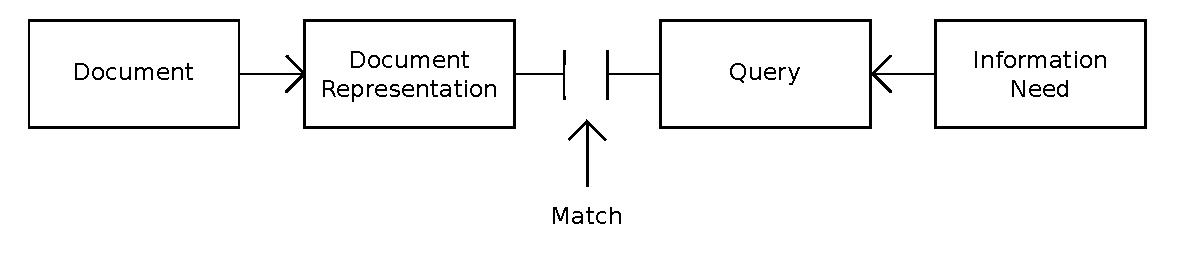
\includegraphics[scale=0.45]{figures/classicIR.pdf}
\end{figure}

After finishing the poster, the group is given a new assignment.
Their second assignment is to write a short play of any historical event that was of special importance for Denmark and then perform the play in front of the class.
This time, the information needed for completing the assignment can not be clearly defined. 
Compared to the previous assignment, it takes much more time.
Estimating the needed time and effort is harder, because the goal is not as clear as it was with the previous assignment.

The students might start by reading the history of Denmark in the Wikipedia.
Along their exporation, they come upon different events and characters that have had an effect in Denmark's history and make new queries regarding the newly-found topics.
The information seeking process described here fits well in what is said of berrypicking behaviour (See Figure \ref{figure_bp}).
In berrypicking behaviour the searcher gets new ideas and new paths to follow as they browse the search results of their search query. In the example, as the students are reading about the 10th century events in Denmark, they might get interested in Harald Bluetooth, the King of Denmark at the time, and begin searching for information of him.  

\begin{figure}[htp] % t=top, h=here, b=bottom, p=separate page, !=place even if ugly
\caption{An evolving berrypicking search. Based on \protect\cite{bates89}. From \protect\cite{march06}.}
\label{figure_bp}
\centering
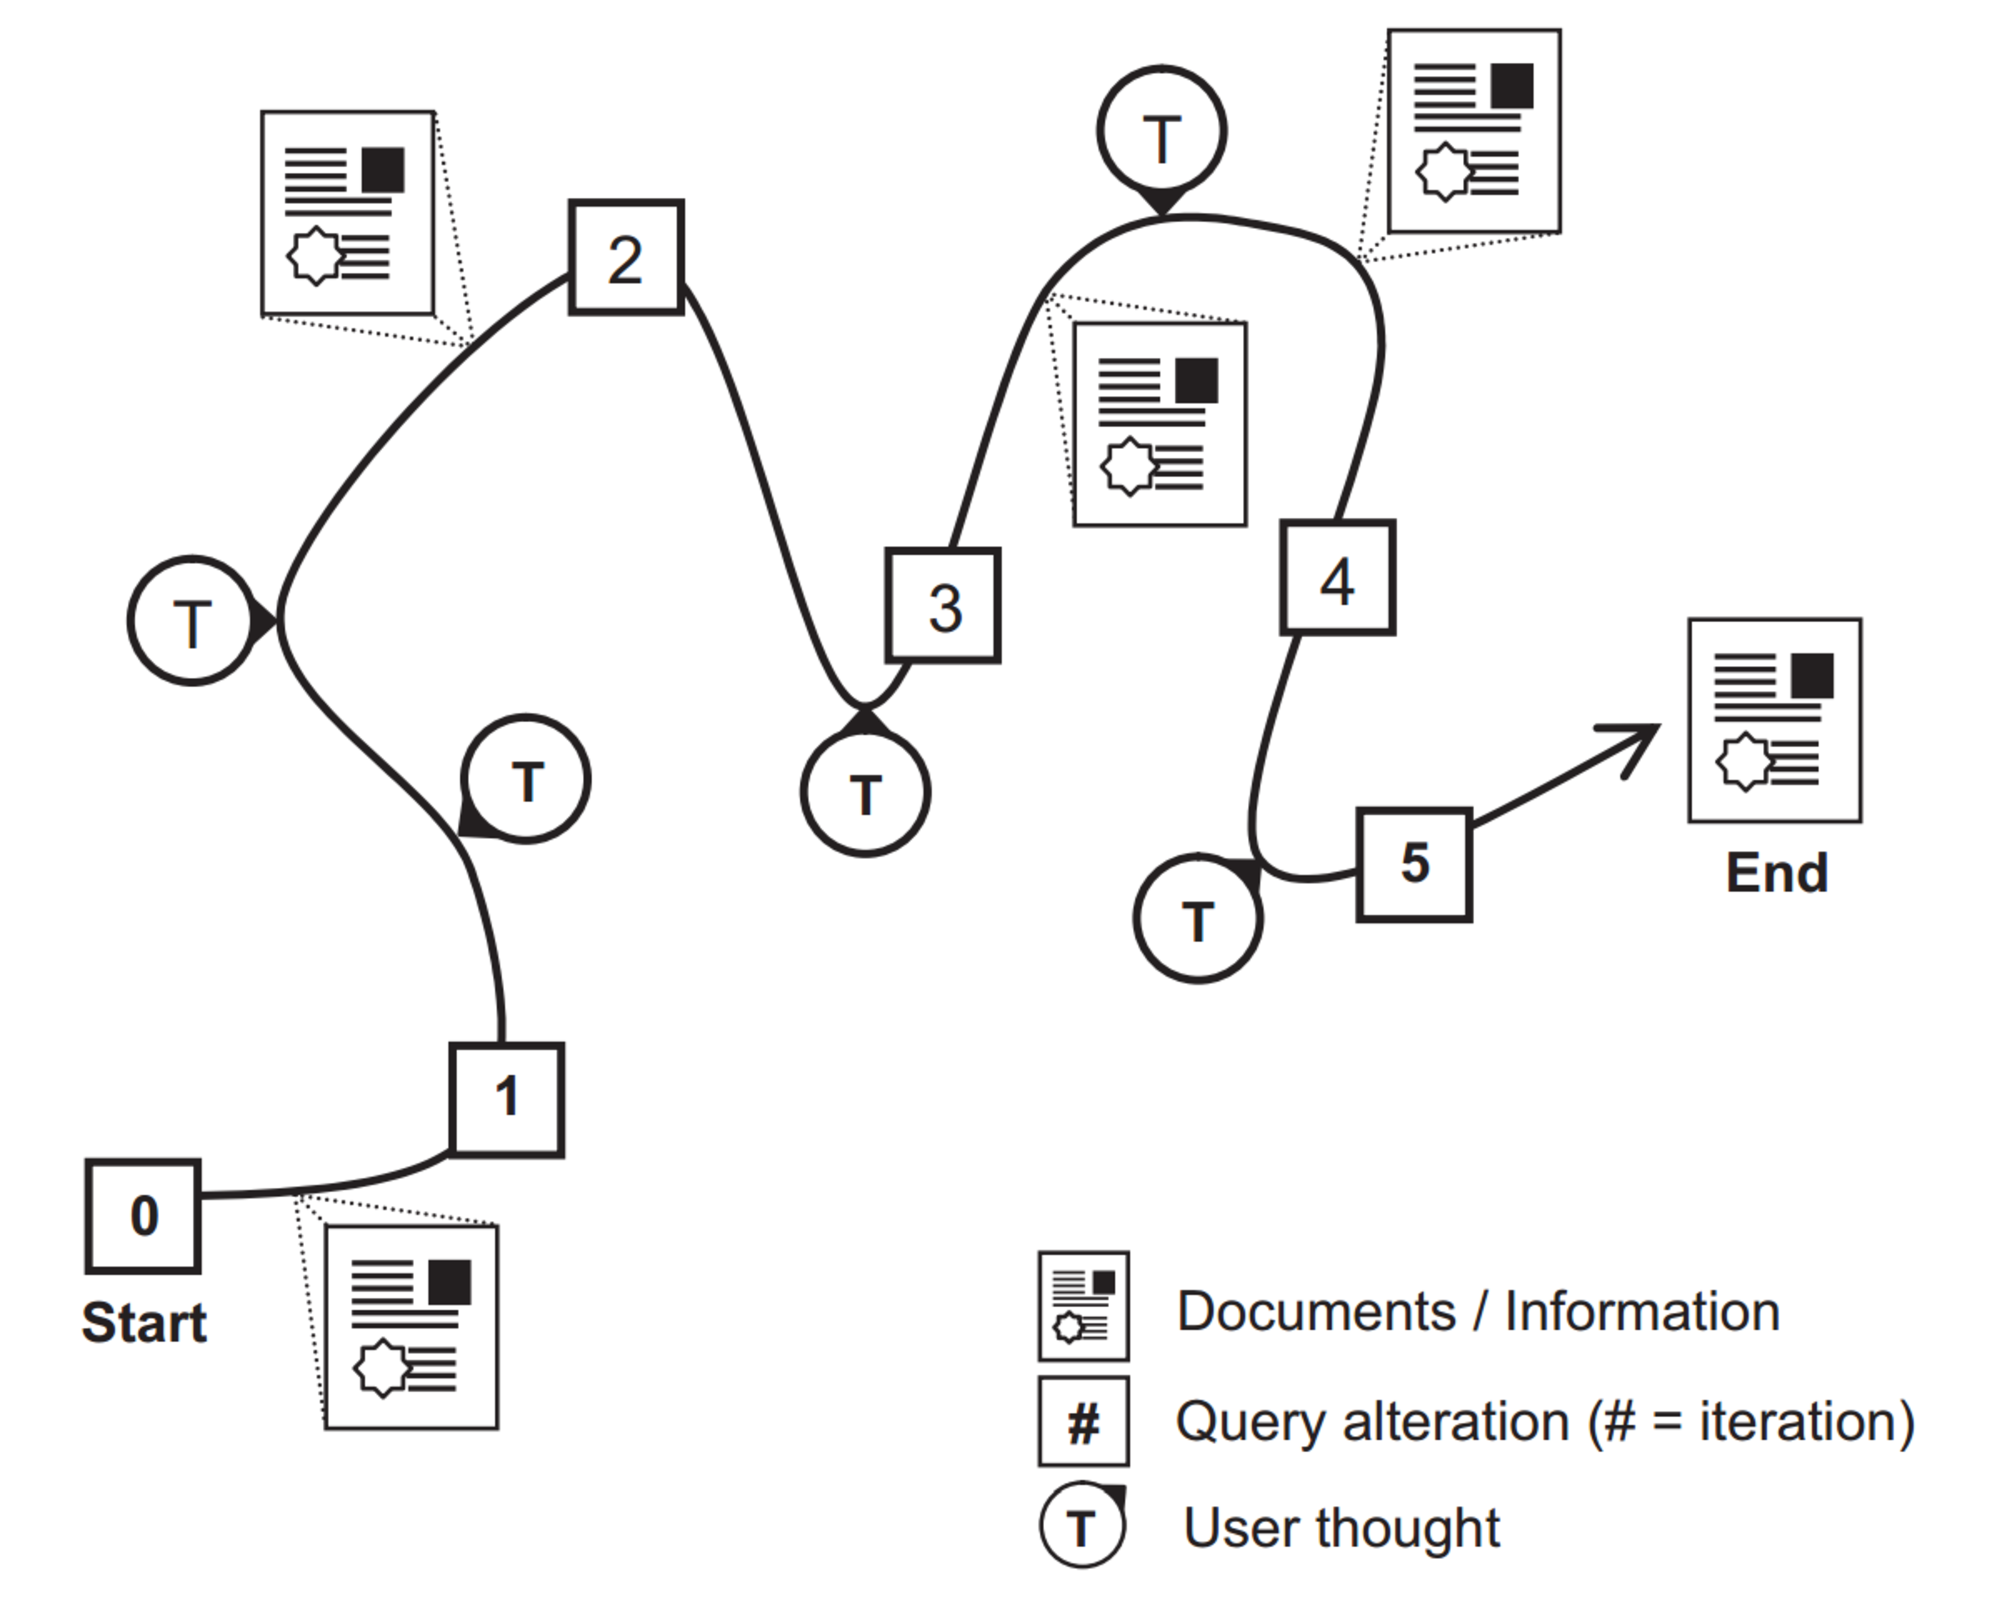
\includegraphics[scale=0.25]{figures/berrypicking.pdf}
\end{figure}

Bates \cite{bates89} describes the berrypicking approach as "evolving search", because during the process the desired outcome may change, as well as the query.

With their now improved knowledge of Danish history, they need to decide which event to depict in their play.
This requires collaboration within the group, which is typical for exploratory search activities.
After decision on the event, the group needs to gather information to be able to write a script for the play.
They have to do some research on the people involved in the selected historical event and if necessary, they must seek for information on what kind of clothes were used in the era the event took place in.
The previously used websites might lack the information they are after so the searchers have to find new sources of information and their search strategies may change.
As seen in Figure \ref{figure_bp}, new information results in query alterations or user thoughts.
Bates \cite{bates90} described a four-level hierarchy of search activities within berrypicking: move, tactic, stratagem and strategy.
Single physical or mental actions by the user are moves, and tactics are a combination of moves. 
Berrypicking could be described as complex combination of moves and tactics, whereas lookup-based information retrieval is a simple set of tactics and moves \cite{white09}.

\begin{figure}[htp] % t=top, h=here, b=bottom, p=separate page, !=place even if ugly
\caption{Different search tasks are split into three overlapping search activities: \textit{lookup}, \textit{learn} and \textit{investigate}. Based on \protect\cite{march06}.}
\label{figure_3clouds}
\centering
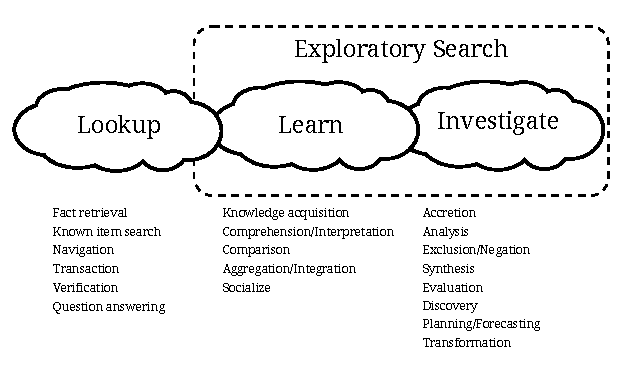
\includegraphics[scale=0.8]{figures/3clouds2.pdf}
\end{figure}

Introduction to exploratory search. See Figure \ref{figure_3clouds}.
\cite{march06}, \cite{white09}, \cite{tvaro11}

The user interface of an exploratory search system should be designed to fulfill the needs of most of its users. More information on what works and doesn't work can usually be collected from system evaluations.
However, evaluating exploratory search systems is difficult, because users have different starting positions. Their knowledge of the domain varies, they are interested in different aspects of the topic and they have previously encountered different information. \cite{kules08}

Exploratory search and iterative search differ. See Figure \ref{figure_IterativeVsExploratory}.

\begin{figure}[htp] % t=top, h=here, b=bottom, p=separate page, !=place even if ugly
\caption{They differ. From \protect\cite{white09}.}
\label{figure_IterativeVsExploratory}
\centering
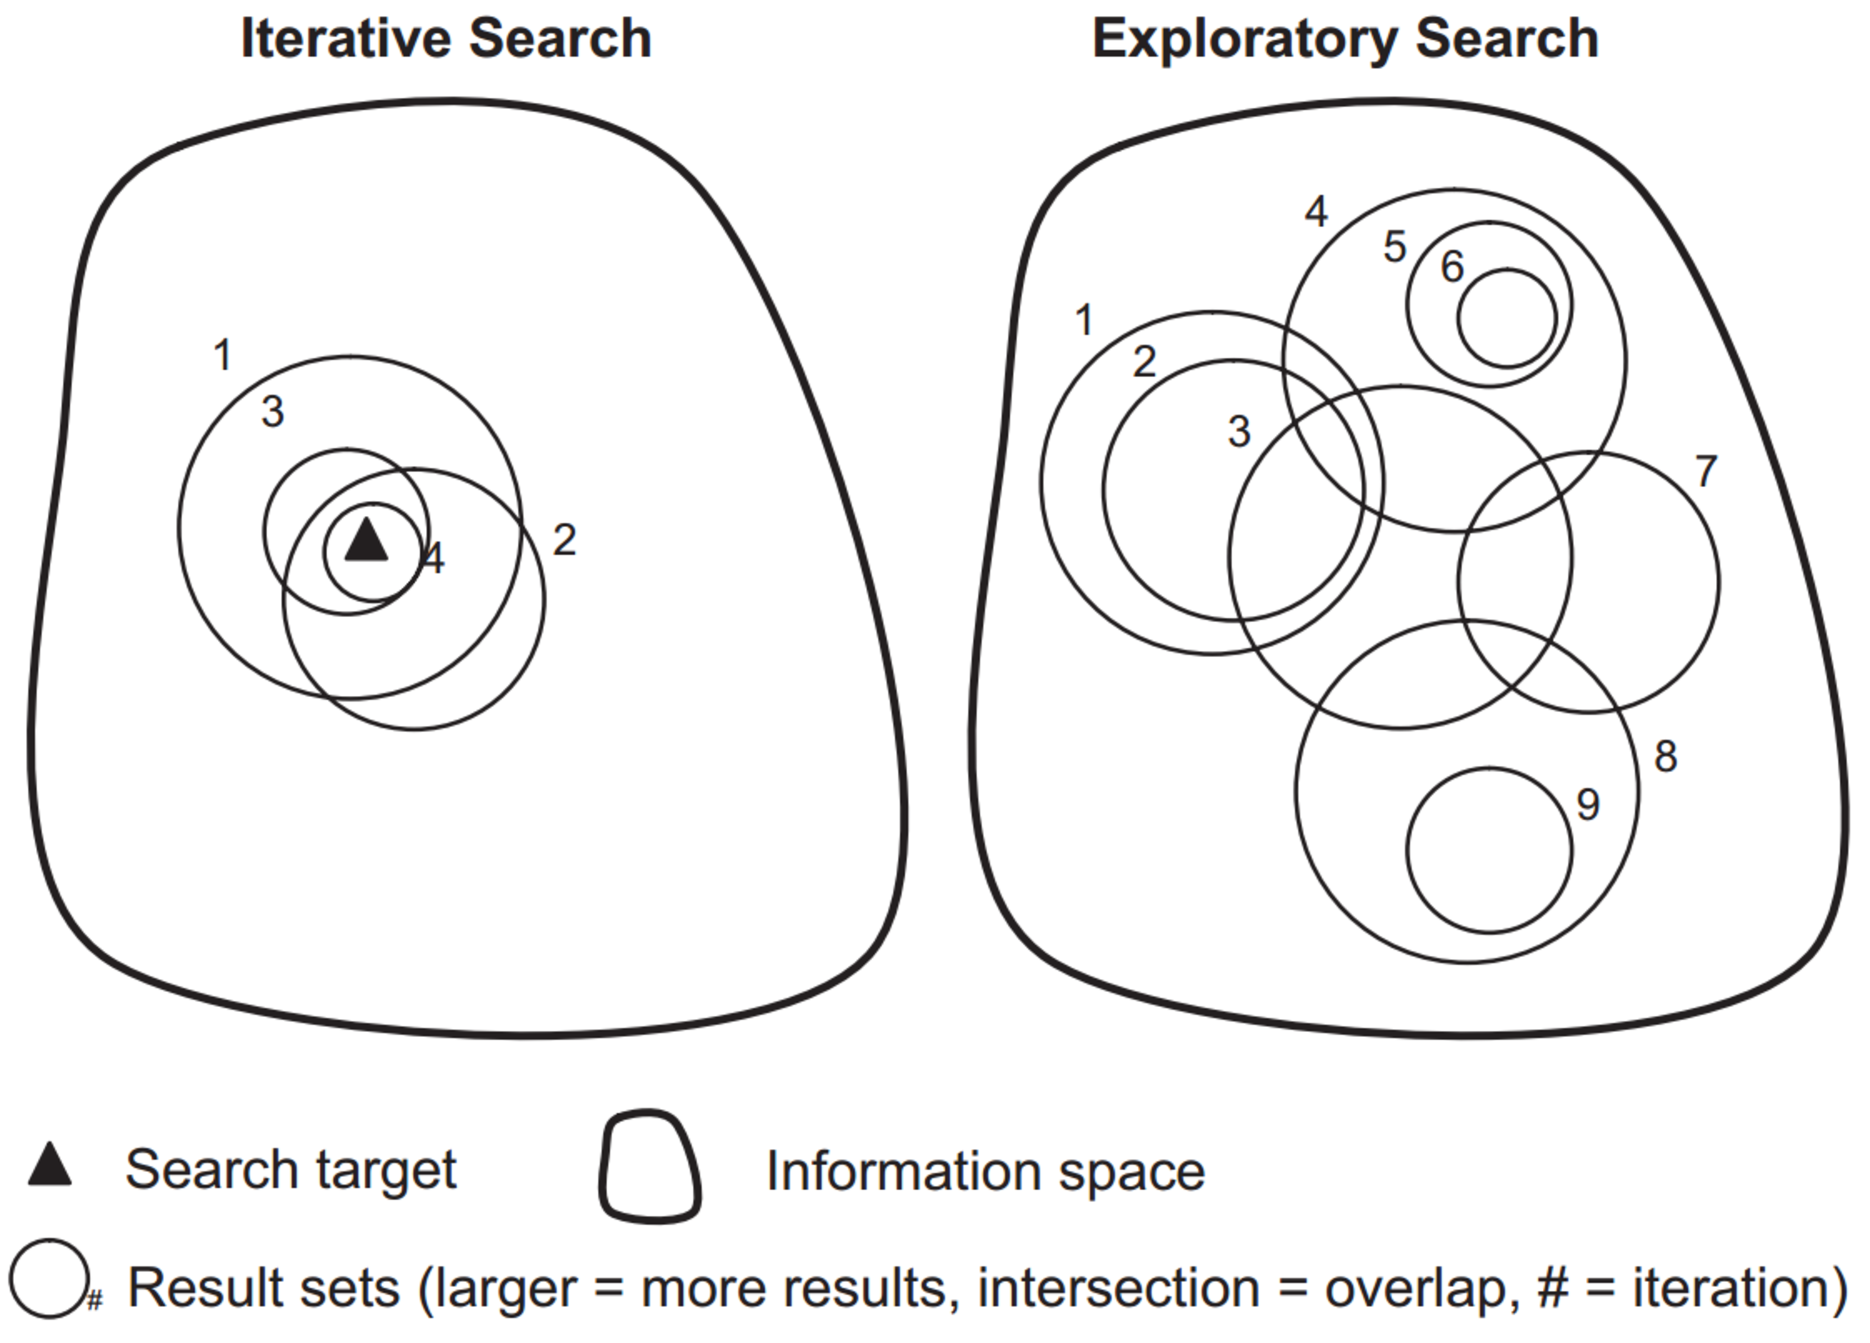
\includegraphics[scale=0.25]{figures/IterativeSearch_vs_ExploratorySearch.pdf}
\end{figure}

Exploratory search tasks can be characterized as either learning oriented or investigative  and they have common aspects like uncertainty, ambiguity and discovery distinguishing them from look-up oriented tasks \cite{kules09}.

